\begin{frame}
\frametitle{AugUCB algorithm (Intuition, Arm pulling)}
\begin{itemize}
%\item We define $\Delta_i = |r_i - \tau| $ . 
\item Like UCB-Imp, AugUCB also divides the time budget $T$ into rounds.
\item At every timestep we pull the arm that minimizes $j\in\argmin_{i\in B_{m}}\Big\lbrace |\hat{r}_{i} - \tau | - 2s_{i}\Big\rbrace$ (like APT). 
\end{itemize}

\begin{figure}
\caption{AugUCB Intuition (Arm pulling)}
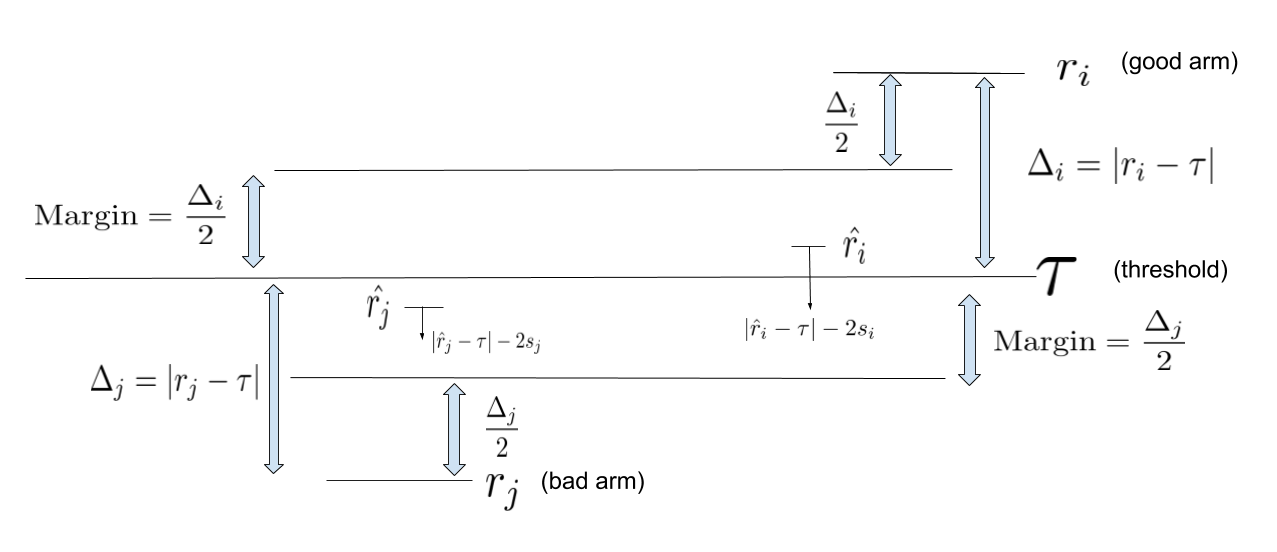
\includegraphics[scale=0.178]{img/SeminarThresholdBandit.png}
\end{figure}
\end{frame}

\begin{frame}
\frametitle{AugUCB algorithm (Intuition, Arm Elimination)}
\begin{itemize}
\item It is risky to eliminate arm $i$ while $\hat{r}_i$ is inside \emph{Margin}. 
\item Confidence interval $s_i$ will make sure arm $i$ is not eliminated while inside Margin with a high probability. 
\end{itemize}

\begin{figure}
\caption{AugUCB Intuition (Arm Elimination)}
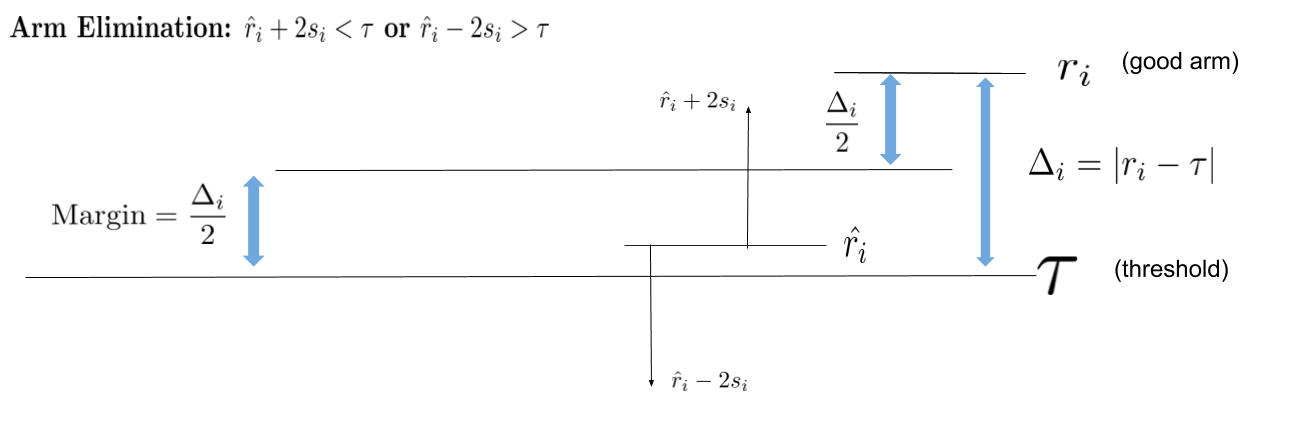
\includegraphics[scale=0.278]{img/ArmElim1.png}
\end{figure}
\end{frame}

\begin{frame}
\frametitle{AugUCB algorithm (Intuition, Arm Elimination)}
\begin{figure}
\caption{AugUCB Intuition (Arm Elimination)}
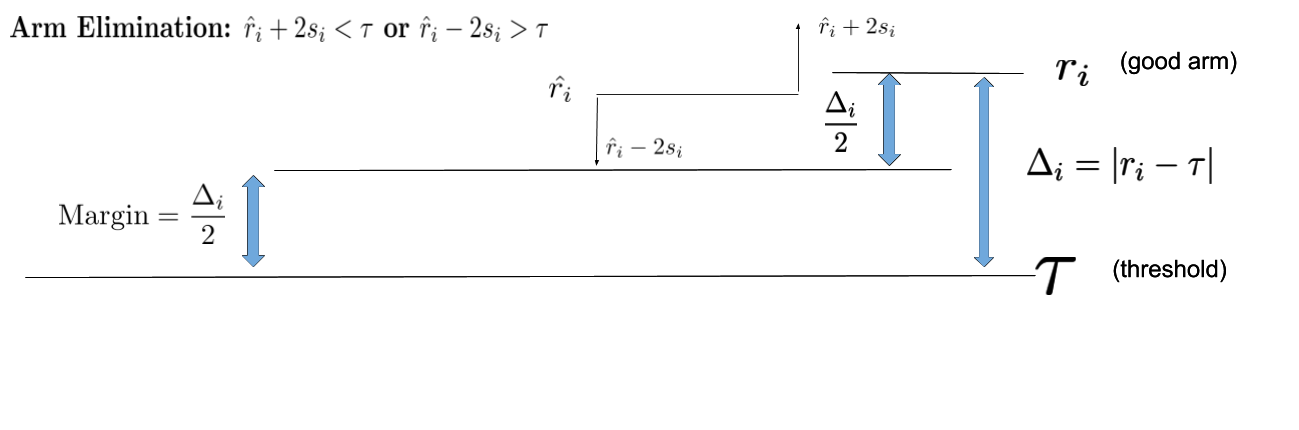
\includegraphics[scale=0.278]{img/ArmElim2.png}
\end{figure}
\end{frame}

\begin{frame}
\frametitle{AugUCB algorithm}
\begin{figure}
\caption{AugUCB Flowchart}
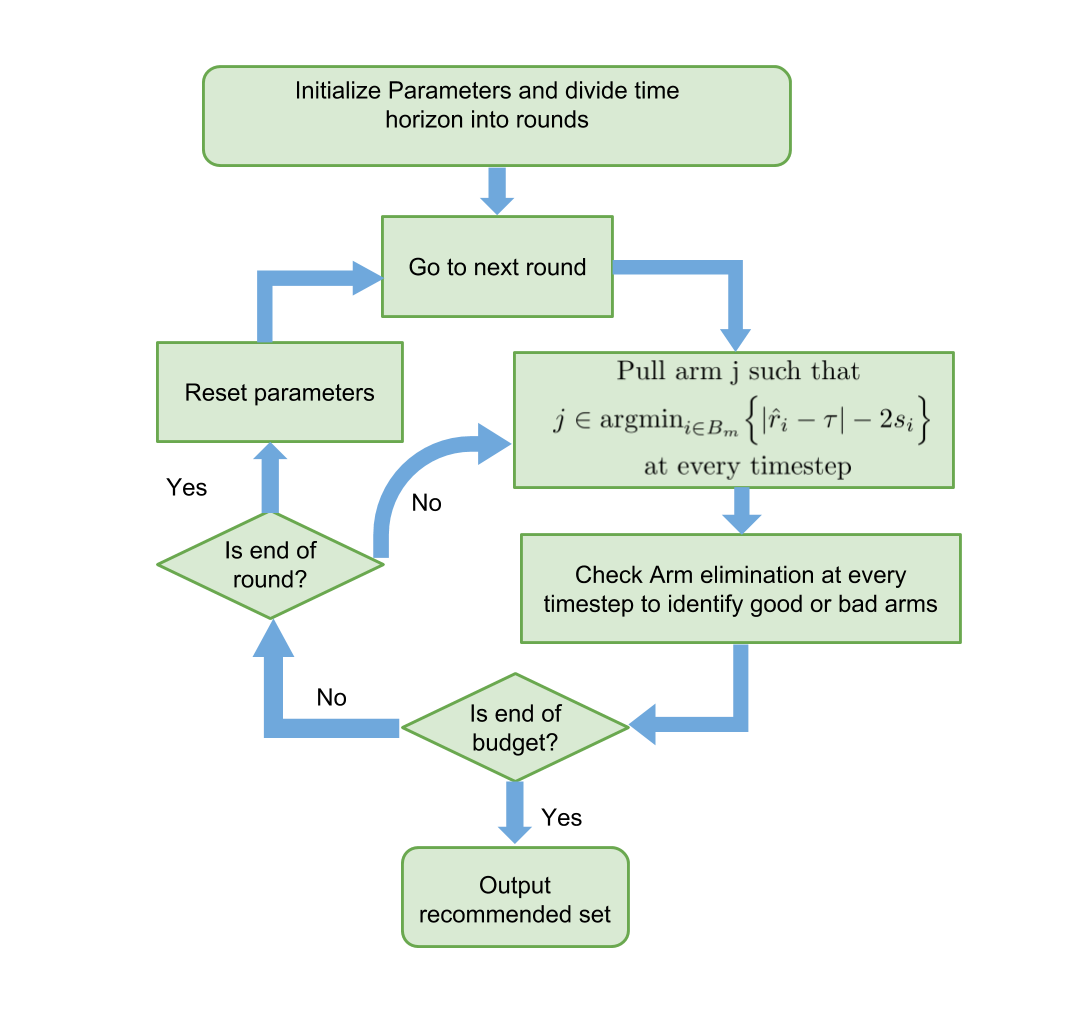
\includegraphics[scale=0.178]{img/AugUCB_flow.png}
\end{figure}
\end{frame}


%\begin{frame}
%\frametitle{AugUCB algorithm}
%\begin{itemize}
%\item<1-> Like UCB-Imp, AugUCB also divides the time budget $T$ into rounds.
%\item<2-> A crucial difference is that in every round instead of pulling all the arms equal number of times we pull the arm that minimizes $j\in\argmin_{i\in B_{m}}\Big\lbrace |\hat{r}_{i} - \tau | - 2s_{i}\Big\rbrace$ (like APT). 
%\item<3-> At every timestep now we run the arm elimination check to eliminate sub-optimal arms.
%\item<4-> At the end of the phase we reset the parameters. 
%\item<5-> Note that the length of the phase, the exploration parameters and the confidence interval term $s_i  = \sqrt{\frac{\rho\psi_m (\hat{v}_{i}+1) \log ( T \epsilon_{m})}{4 n_{i}}}$ are set through detailed theoretical analysis. 
%\end{itemize}
%\end{frame}

\begin{frame}
\frametitle{AugUCB parameter initialization}
\begin{figure}
\caption{AugUCB parameter initialization}
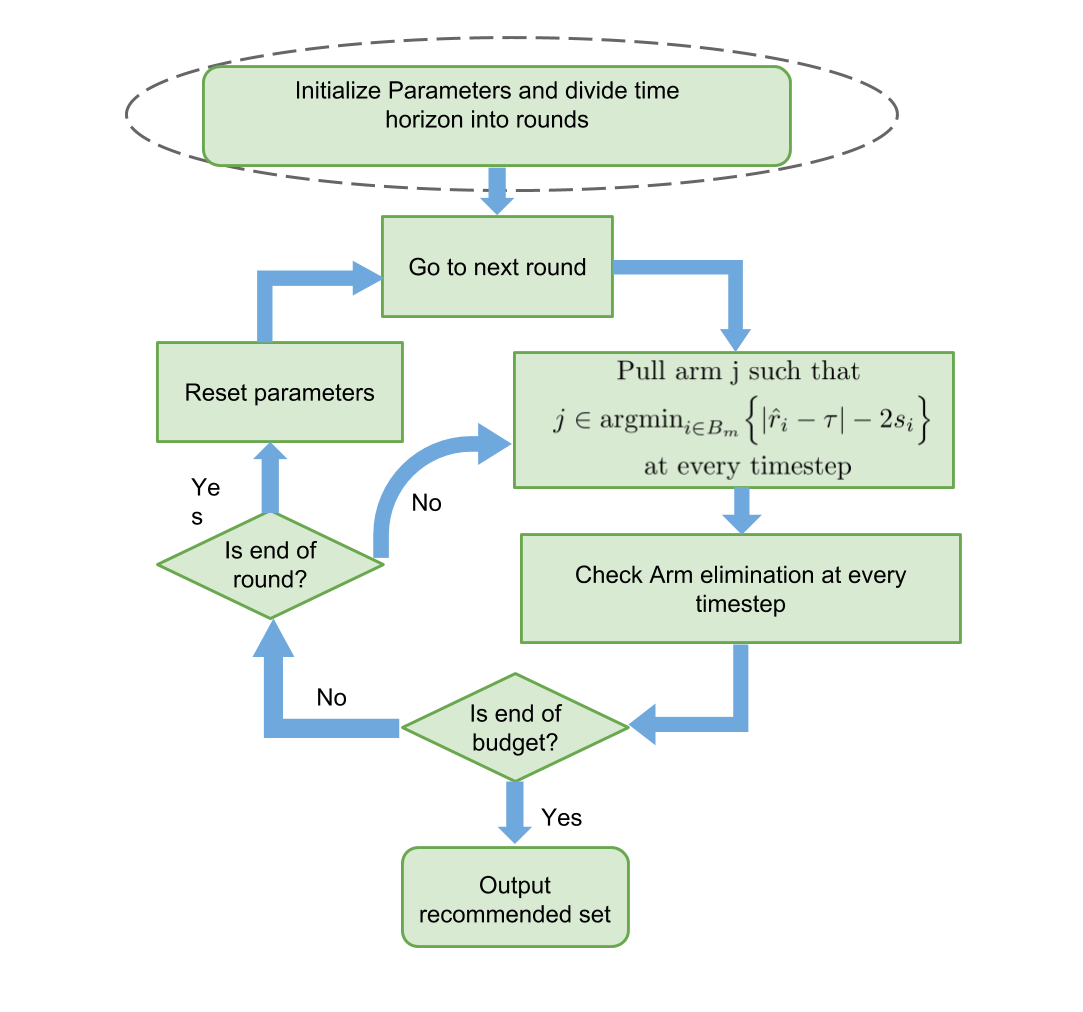
\includegraphics[scale=0.178]{img/AugUCB_flow_param.png}
\end{figure}
\end{frame}


\begin{frame}
\frametitle{Parameter initialization}
\begin{itemize}
\item<1-> We define $\ell_{0} =\left\lceil \frac{2\psi_0\log( T\epsilon_{0})}{\epsilon_{0}} \right\rceil$ as the budget allocated to each arm in a round.
\item<2-> The first round gets divided into $N_{0}=K\ell_{0}$
\item<3-> We define a large exploration regulatory factor $\psi_{0}=\frac{T\epsilon_{0}}{128\Big(\log(\frac{3}{16}K\log K)\Big)^2}$.
%\item<1-> M&=\left\lfloor \frac{1}{2}\log_{2} \frac{T}{e}\right\rfloor; 
%\hspace{2mm}\psi_{0}=\frac{T\epsilon_{0}}{128\Big(\log(\frac{3}{16}K\log K)\Big)^2}; \\
%\ell_{0}&=\left\lceil \frac{2\psi_0\log( T\epsilon_{0})}{\epsilon_{0}} \right\rceil ;
%\hspace{2mm}N_{0}=K\ell_{0}
%\item<2->
\end{itemize}
\end{frame}

\begin{frame}
\frametitle{AugUCB arm pull}
\begin{figure}
\caption{AugUCB arm pulln}
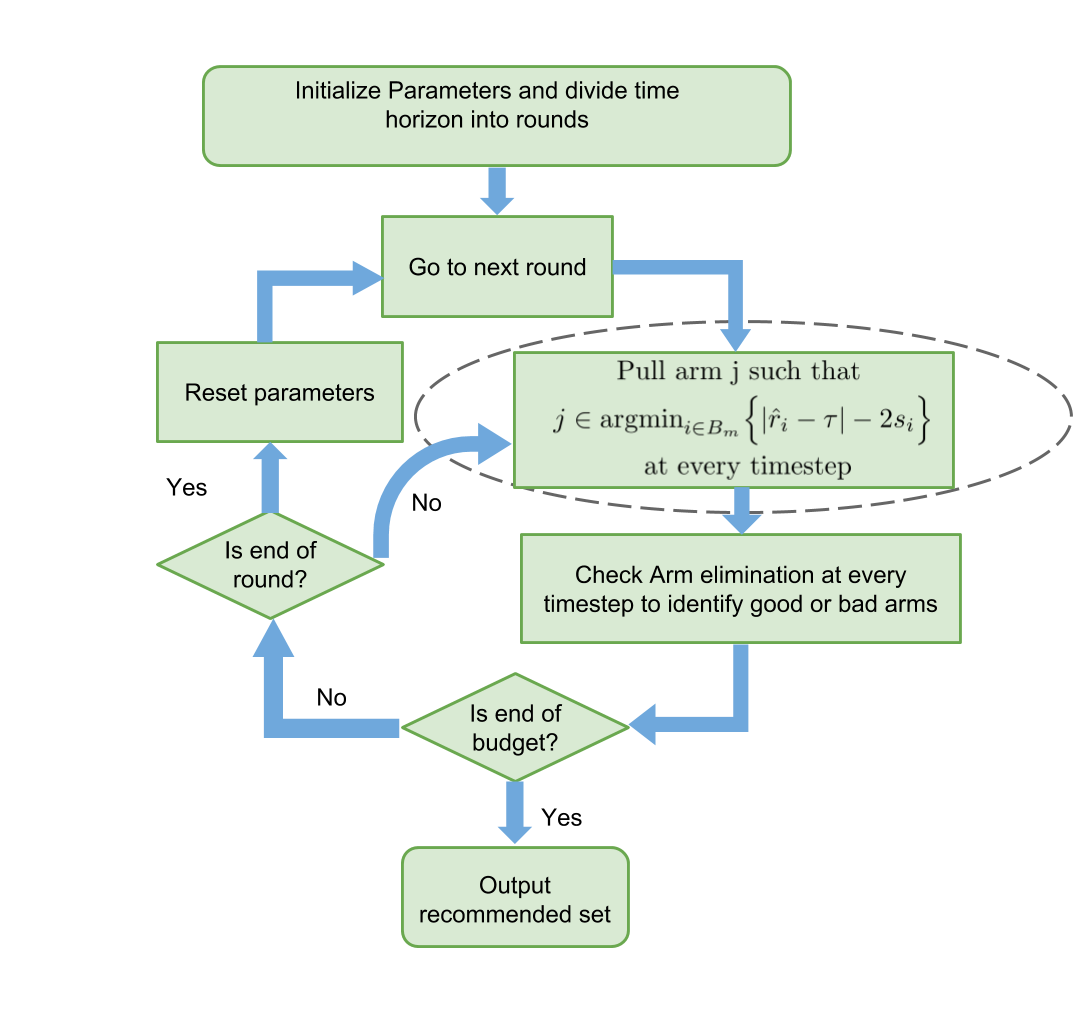
\includegraphics[scale=0.178]{img/AugUCB_flow_armpull.png}
\end{figure}
\end{frame}

\begin{frame}
\frametitle{Arm pull}
\begin{itemize}
\item<1-> We pull the arm that minimizes $j\in\argmin_{i\in B_{m}}\Big\lbrace |\hat{r}_{i} - \tau | - 2s_{i}\Big\rbrace$
\item<2-> We define the confidence interval $s_i  = \sqrt{\frac{\rho\psi_m (\hat{v}_{i}+1) \log ( T \epsilon_{m})}{4 n_{i}}}$.
\item<3-> $s_i$ decreases with more $n_i$ and $\psi_m$ and $\rho$ ensures that it decreases at a correct rate.
\item<4-> Note that $\hat{v}_i$ estimated variance in $s_i$ makes the algorithm pull the arm which shows more variance. 
\end{itemize}
\end{frame}

\begin{frame}
\frametitle{AugUCB arm elimination}
\begin{figure}
\caption{AugUCB arm elimination}
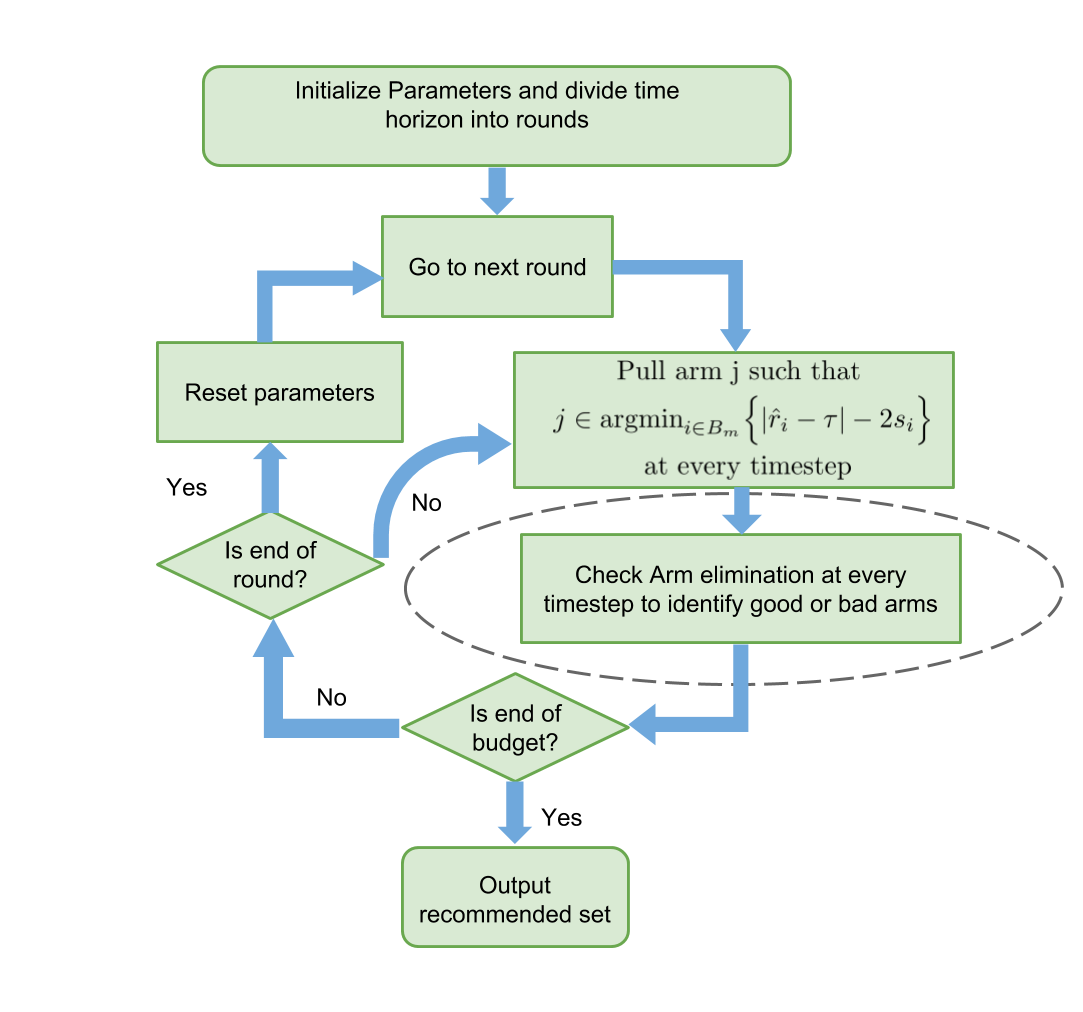
\includegraphics[scale=0.178]{img/AugUCB_flow_elim.png}
\end{figure}
\end{frame}


\begin{frame}
\frametitle{Arm elim}
\begin{itemize}
\item<1-> Arm elimination condition is checked at every timestep.
\item<2-> It eliminated arm which are above or below margin.
\item<3-> Re-allocates the remaining budget for surviving arms. 
\end{itemize}
\end{frame}


\begin{frame}
\frametitle{AugUCB parameter reset}
\begin{figure}
\caption{AugUCB parameter reset}
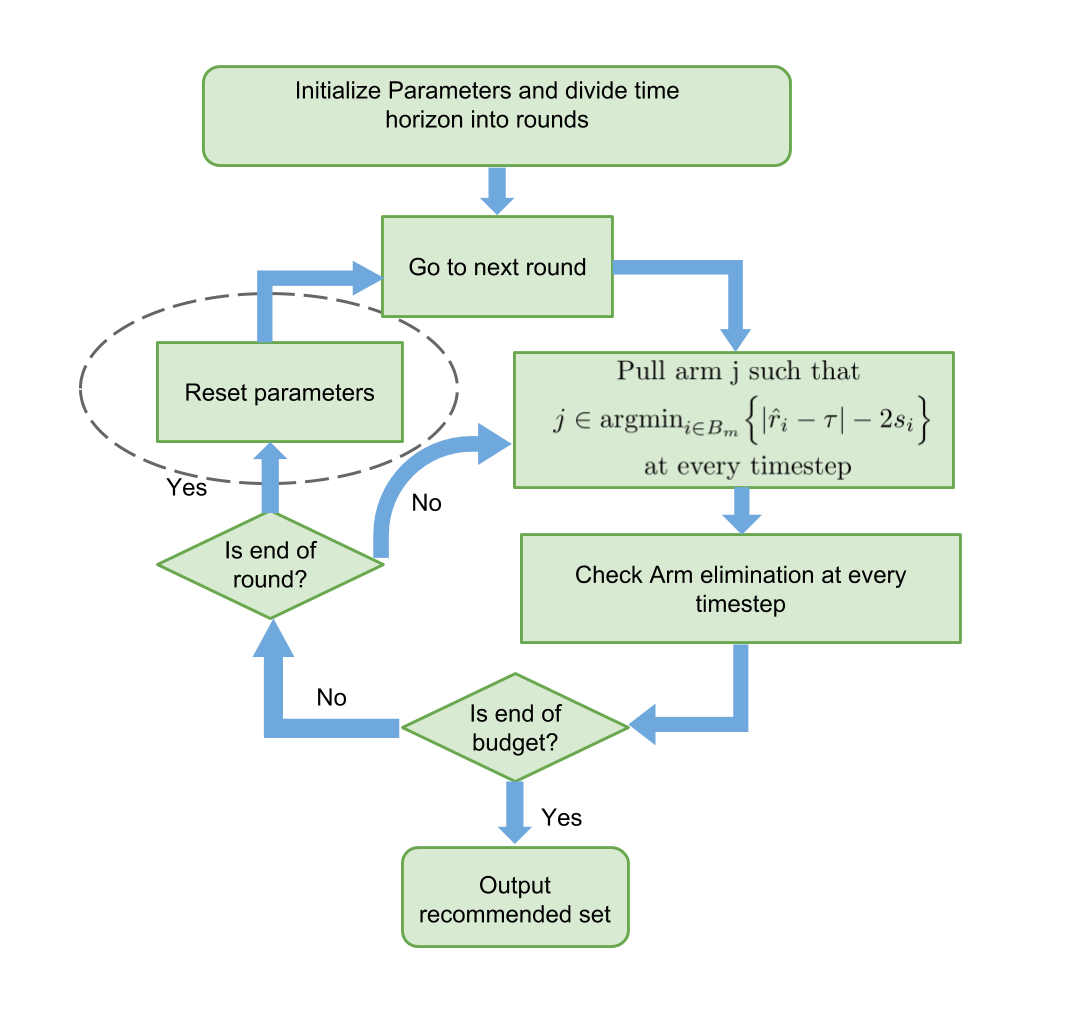
\includegraphics[scale=0.178]{img/AugUCB_flow_reset.png}
\end{figure}
\end{frame}


\begin{frame}
\frametitle{AugUCB parameter reset}
\begin{itemize}
\item<1-> Reduce the exploration factor as time progresses.
\item<2-> Recalculate the budget for each surviving arms.
\item<3-> Recalculate the length of each round on the number of surviving arms.
\end{itemize}
\end{frame}

%\begin{frame}[allowframebreaks]
%\frametitle{AugUCB algorithm}
%%\begin{algorithm}[H]
%%\caption{AugUCB}
%%\label{alg:augucb}
%\begin{algorithmic}
%\State {\bf Input:} Time budget $T$; parameter $\rho$; threshold $\tau$
%\State {\bf Initialization:} $B_{0}=\mathcal{A}$; $m=0$; $\epsilon_{0}=1$;
%\begin{small}
%\begin{align*}
%M&=\left\lfloor \frac{1}{2}\log_{2} \frac{T}{e}\right\rfloor; 
%\hspace{2mm}\psi_{0}=\frac{T\epsilon_{0}}{128\Big(\log(\frac{3}{16}K\log K)\Big)^2}; \\
%\ell_{0}&=\left\lceil \frac{2\psi_0\log( T\epsilon_{0})}{\epsilon_{0}} \right\rceil ;
%\hspace{2mm}N_{0}=K\ell_{0}
%\end{align*}
%\end{small}
%\State Pull each arm once
%\vspace{-3mm}
%\State \For{$t=K+1,..,T$}
%\State Pull arm $j\in\argmin_{i\in B_{m}}\Big\lbrace |\hat{r}_{i} - \tau | - 2s_{i}\Big\rbrace$
%\vspace{-4.5mm}
%\State \For{$i\in B_m$}
%\vspace{-4.5mm}
%\State \If{$(\hat{r}_{i} + s_i  < \tau - s_i)$ or $(\hat{r}_{i} - s_i > \tau + s_i)$}
%\State $B_m\leftarrow B_m\backslash\{i\}$\hspace{4mm} (Arm deletion)
%\EndIf
%\EndFor
%\vspace{-2mm}
%\State \If{$t\geq N_{m}$ and $m \leq M$}
%%\ResetParam
%\State \textbf{Reset Parameters}
%\State $\epsilon_{m+1}\leftarrow\frac{\epsilon_{m}}{2}$
%\State $B_{m+1} \leftarrow B_{m}$
%\State $\psi_{m+1}\leftarrow \frac{T\epsilon_{m+1}}{128(\log(\frac{3}{16}K\log K))^{2}}$
%\State $\ell_{m+1}\leftarrow\left\lceil \frac{2\psi_{m+1}\log( T\epsilon_{m+1})}{\epsilon_{m+1}} \right\rceil$
%\State $N_{m+1} \leftarrow t + |B_{m+1}|\ell_{m+1}$
%\State $m \leftarrow m+1$
%\EndIf
%\EndFor
%\State \textbf{Output:} $\hat{S}_{\tau}=\lbrace i: \hat{r}_{i}\geq \tau \rbrace$.
%\end{algorithmic}
%%\end{algorithm}
%\end{frame}